\chapter{Numerical results for the $\Hd$ anyon chain}
\label{app:H3chain}

In the following, we depict the entropy landscape for the Hamiltonian described in \cref{sec:H3chain}:
	\begin{equation}
		H=-\sum_i \cos\psi\ p_i^{(\mathbf{1})}+\sin\psi\cos\theta\  p_i^{(\rho)}+\sin\psi\sin\theta\cos\varphi\ p_i^{(\alpharho)}+\sin\psi\sin\theta\sin\varphi\  p_i^{(\alphastarrho)}.
	\end{equation}
Each diagram corresponds to a fixed value of $\varphi$. The interval $[0,\pi]$ is always divided into $16$ pieces in order to generate data points. The resulting landscape is then visualised by a contour plot, where dark colours correspond to a low entropy and bright colours correspond to a high entropy.

\noindent
\begin{minipage}{0.48\textwidth}
	\centering
	\begin{figure}[H]
		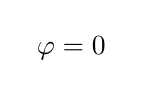
\begin{tikzpicture}
		\node at (0,0) {$\varphi=0$};
		\end{tikzpicture}\\
		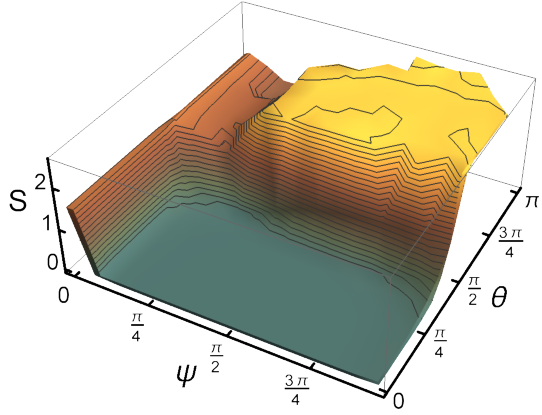
\includegraphics[width=1\textwidth]{data/Plots/Plot0.pdf}
	\end{figure}
\end{minipage}\hspace{10pt}
\begin{minipage}{0.48\textwidth}
	\centering
	\begin{figure}[H]
		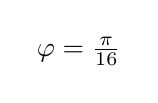
\begin{tikzpicture}
		\node at (0,0) {$\varphi=\frac{\pi}{16}$};
		\end{tikzpicture}\\
		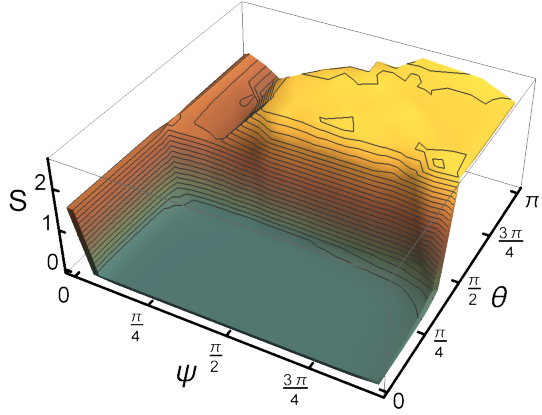
\includegraphics[width=1\textwidth]{data/Plots/Plot1.pdf}
	\end{figure}
\end{minipage}
\vspace{10pt}

\noindent
\begin{minipage}{0.48\textwidth}
	\centering
	\begin{figure}[H]
		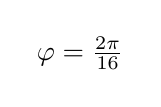
\begin{tikzpicture}
		\node at (0,0) {$\varphi=\frac{2\pi}{16}$};
		\end{tikzpicture}\\
		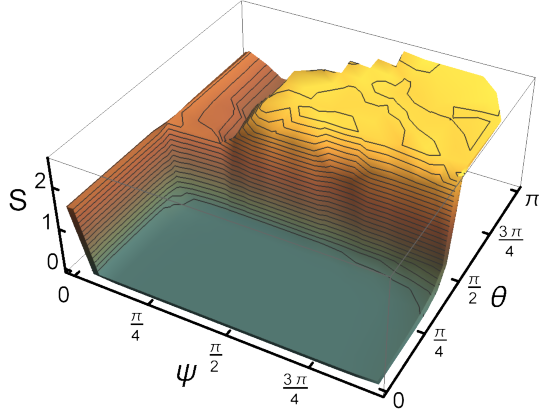
\includegraphics[width=1\textwidth]{data/Plots/Plot2.pdf}
	\end{figure}
\end{minipage}\hspace{10pt}
\begin{minipage}{0.48\textwidth}
	\centering
	\begin{figure}[H]
		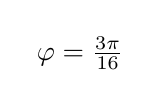
\begin{tikzpicture}
		\node at (0,0) {$\varphi=\frac{3\pi}{16}$};
		\end{tikzpicture}\\
		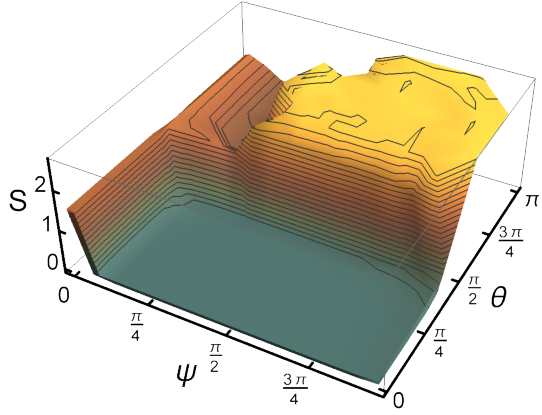
\includegraphics[width=1\textwidth]{data/Plots/Plot3.pdf}
	\end{figure}
\end{minipage}
\vspace{10pt}

\noindent
\begin{minipage}{0.48\textwidth}
	\centering
	\begin{figure}[H]
		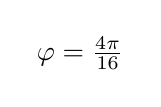
\begin{tikzpicture}
		\node at (0,0) {$\varphi=\frac{4\pi}{16}$};
		\end{tikzpicture}\\
		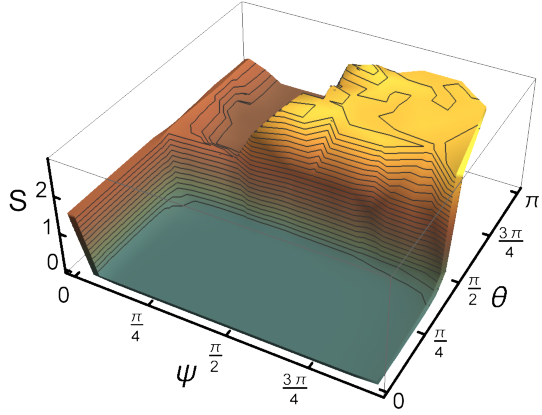
\includegraphics[width=1\textwidth]{data/Plots/Plot4.pdf}
	\end{figure}
\end{minipage}\hspace{10pt}
\begin{minipage}{0.48\textwidth}
	\centering
	\begin{figure}[H]
		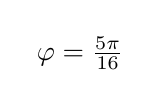
\begin{tikzpicture}
		\node at (0,0) {$\varphi=\frac{5\pi}{16}$};
		\end{tikzpicture}\\
		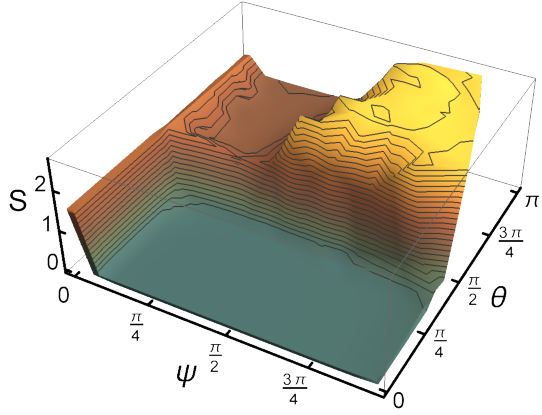
\includegraphics[width=1\textwidth]{data/Plots/Plot5.pdf}
	\end{figure}
\end{minipage}
\vspace{10pt}

\noindent
\begin{minipage}{0.48\textwidth}
	\centering
	\begin{figure}[H]
		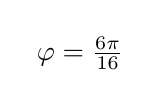
\begin{tikzpicture}
		\node at (0,0) {$\varphi=\frac{6\pi}{16}$};
		\end{tikzpicture}\\
		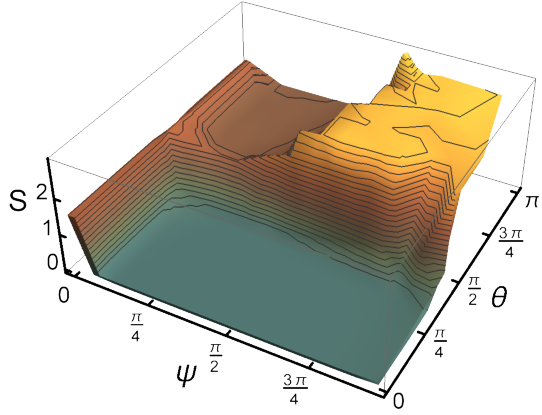
\includegraphics[width=1\textwidth]{data/Plots/Plot6.pdf}
	\end{figure}
\end{minipage}\hspace{10pt}
\begin{minipage}{0.48\textwidth}
	\centering
	\begin{figure}[H]
		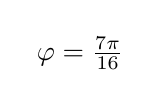
\begin{tikzpicture}
		\node at (0,0) {$\varphi=\frac{7\pi}{16}$};
		\end{tikzpicture}\\
		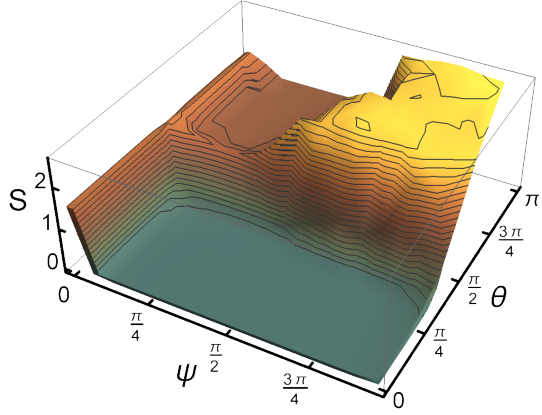
\includegraphics[width=1\textwidth]{data/Plots/Plot7.pdf}
	\end{figure}
\end{minipage}
\vspace{10pt}

\noindent
\begin{minipage}{0.48\textwidth}
	\centering
	\begin{figure}[H]
		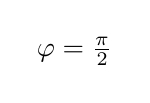
\begin{tikzpicture}
		\node at (0,0) {$\varphi=\frac{\pi}{2}$};
		\end{tikzpicture}\\
		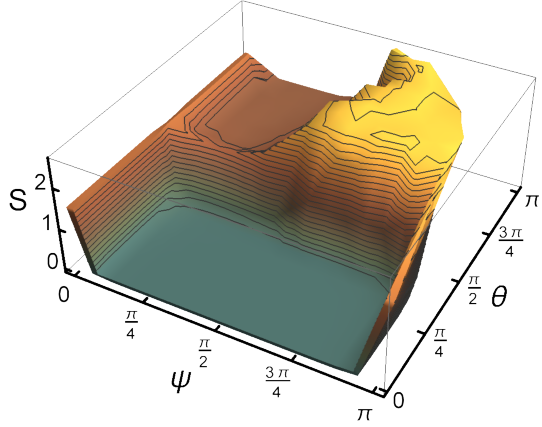
\includegraphics[width=1\textwidth]{data/Plots/Plot8.pdf}
	\end{figure}
\end{minipage}\hspace{10pt}
\begin{minipage}{0.48\textwidth}
	\centering
	\begin{figure}[H]
		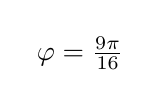
\begin{tikzpicture}
		\node at (0,0) {$\varphi=\frac{9\pi}{16}$};
		\end{tikzpicture}\\
		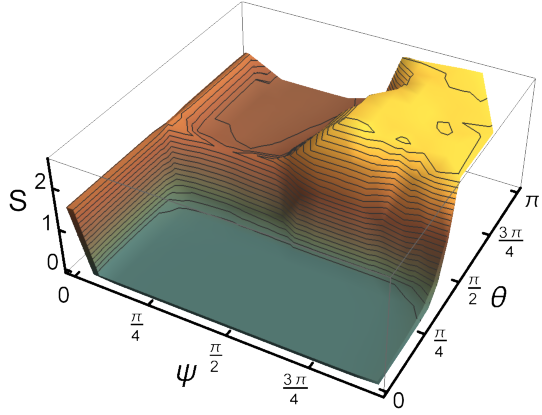
\includegraphics[width=1\textwidth]{data/Plots/Plot9.pdf}
	\end{figure}
\end{minipage}
\vspace{10pt}

\noindent
\begin{minipage}{0.48\textwidth}
	\centering
	\begin{figure}[H]
		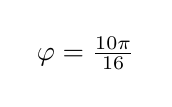
\begin{tikzpicture}
		\node at (0,0) {$\varphi=\frac{10\pi}{16}$};
		\end{tikzpicture}\\
		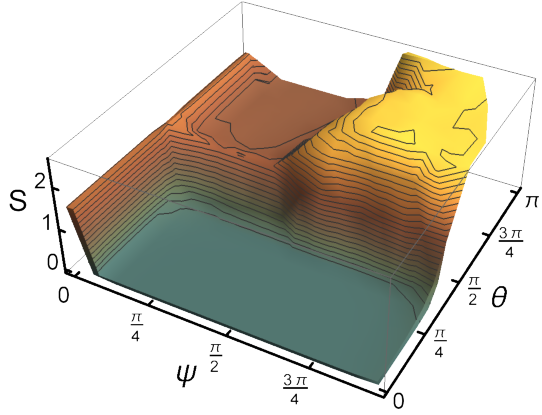
\includegraphics[width=1\textwidth]{data/Plots/Plot10.pdf}
	\end{figure}
\end{minipage}\hspace{10pt}
\begin{minipage}{0.48\textwidth}
	\centering
	\begin{figure}[H]
		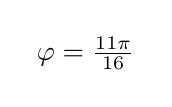
\begin{tikzpicture}
		\node at (0,0) {$\varphi=\frac{11\pi}{16}$};
		\end{tikzpicture}\\
		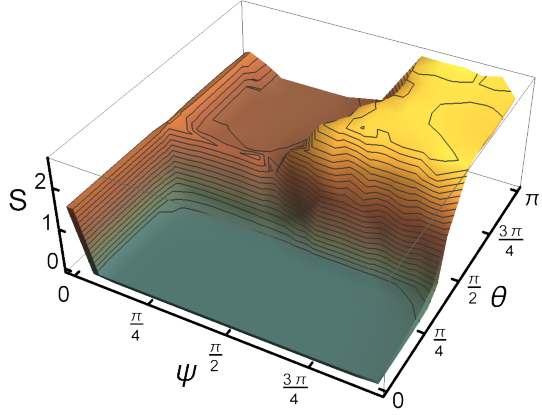
\includegraphics[width=1\textwidth]{data/Plots/Plot11.pdf}
	\end{figure}
\end{minipage}
\vspace{10pt}

\noindent
\begin{minipage}{0.48\textwidth}
	\centering
	\begin{figure}[H]
		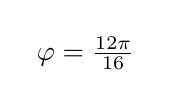
\begin{tikzpicture}
		\node at (0,0) {$\varphi=\frac{12\pi}{16}$};
		\end{tikzpicture}\\
		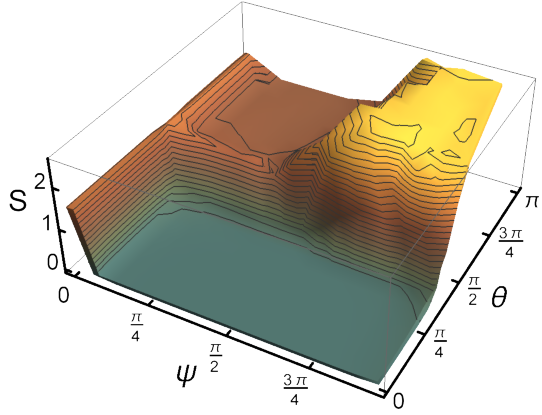
\includegraphics[width=1\textwidth]{data/Plots/Plot12.pdf}
	\end{figure}
\end{minipage}\hspace{10pt}
\begin{minipage}{0.48\textwidth}
	\centering
	\begin{figure}[H]
		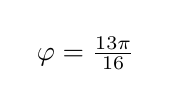
\begin{tikzpicture}
		\node at (0,0) {$\varphi=\frac{13\pi}{16}$};
		\end{tikzpicture}\\
		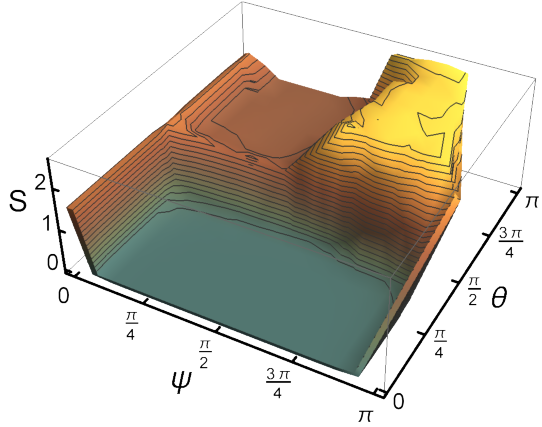
\includegraphics[width=1\textwidth]{data/Plots/Plot13.pdf}
	\end{figure}
\end{minipage}
\vspace{10pt}

\noindent
\begin{minipage}{0.48\textwidth}
	\centering
	\begin{figure}[H]
		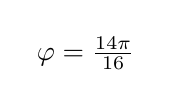
\begin{tikzpicture}
		\node at (0,0) {$\varphi=\frac{14\pi}{16}$};
		\end{tikzpicture}\\
		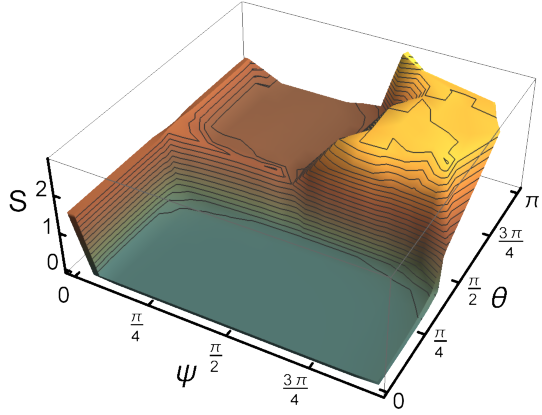
\includegraphics[width=1\textwidth]{data/Plots/Plot14.pdf}
	\end{figure}
\end{minipage}\hspace{10pt}
\begin{minipage}{0.48\textwidth}
	\centering
	\begin{figure}[H]
		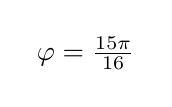
\begin{tikzpicture}
		\node at (0,0) {$\varphi=\frac{15\pi}{16}$};
		\end{tikzpicture}\\
		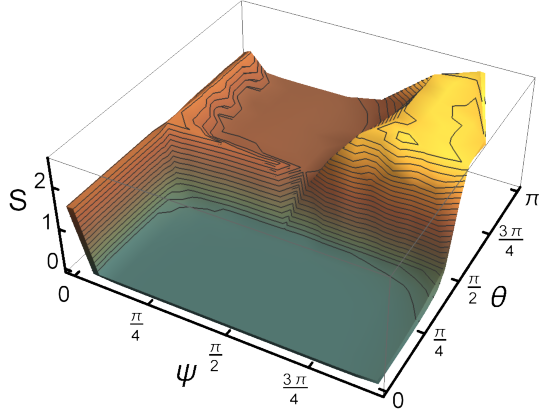
\includegraphics[width=1\textwidth]{data/Plots/Plot15.pdf}
	\end{figure}
\end{minipage}
\vspace{10pt}

\noindent
\begin{minipage}{0.48\textwidth}
	\centering
	\begin{figure}[H]
		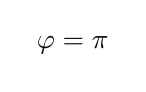
\begin{tikzpicture}
		\node at (0,0) {$\varphi=\pi$};
		\end{tikzpicture}\\
		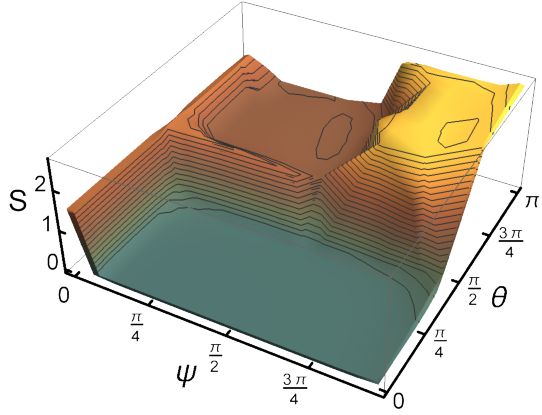
\includegraphics[width=1\textwidth]{data/Plots/Plot16.pdf}
	\end{figure}
\end{minipage}\hspace{10pt}
\begin{minipage}{0.48\textwidth}
	\centering
	\begin{figure}[H]
		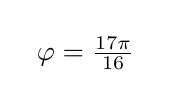
\begin{tikzpicture}
		\node at (0,0) {$\varphi=\frac{17\pi}{16}$};
		\end{tikzpicture}\\
		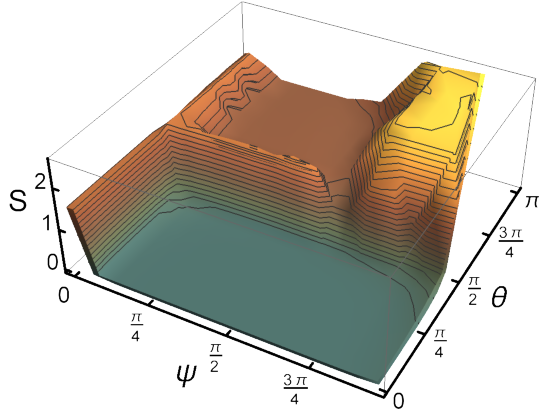
\includegraphics[width=1\textwidth]{data/Plots/Plot17.pdf}
	\end{figure}
\end{minipage}
\vspace{10pt}

\noindent
\begin{minipage}{0.48\textwidth}
	\centering
	\begin{figure}[H]
		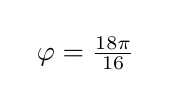
\begin{tikzpicture}
		\node at (0,0) {$\varphi=\frac{18\pi}{16}$};
		\end{tikzpicture}\\
		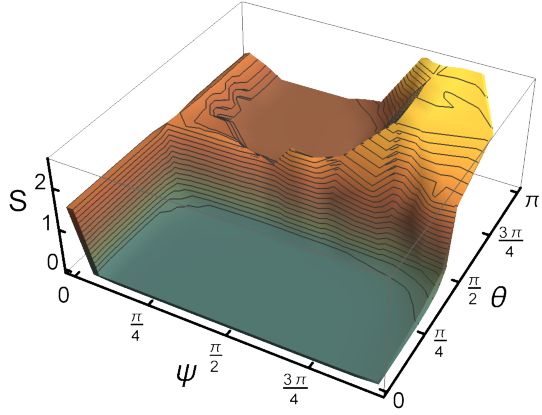
\includegraphics[width=1\textwidth]{data/Plots/Plot18.pdf}
	\end{figure}
\end{minipage}\hspace{10pt}
\begin{minipage}{0.48\textwidth}
	\centering
	\begin{figure}[H]
		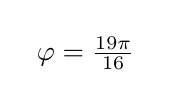
\begin{tikzpicture}
		\node at (0,0) {$\varphi=\frac{19\pi}{16}$};
		\end{tikzpicture}\\
		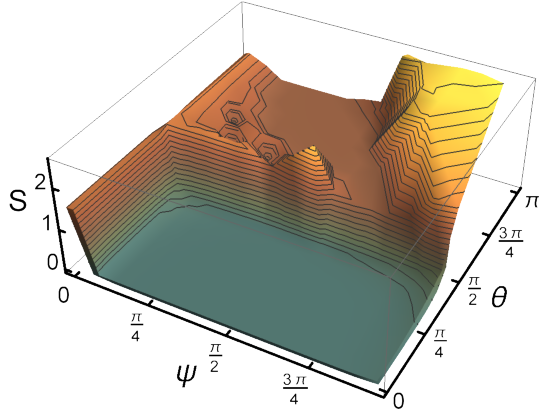
\includegraphics[width=1\textwidth]{data/Plots/Plot19.pdf}
	\end{figure}
\end{minipage}
\vspace{10pt}

\noindent
\begin{minipage}{0.48\textwidth}
	\centering
	\begin{figure}[H]
		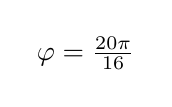
\begin{tikzpicture}
		\node at (0,0) {$\varphi=\frac{20\pi}{16}$};
		\end{tikzpicture}\\
		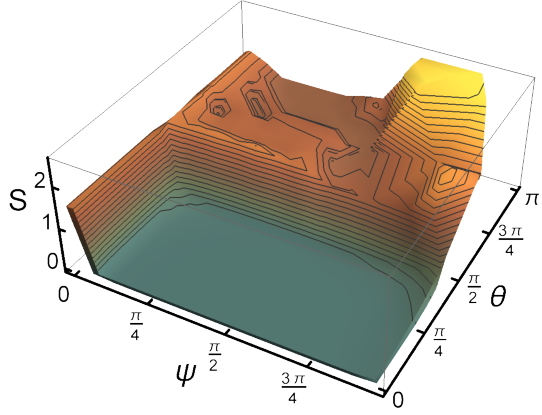
\includegraphics[width=1\textwidth]{data/Plots/Plot20.pdf}
	\end{figure}
\end{minipage}\hspace{10pt}
\begin{minipage}{0.48\textwidth}
	\centering
	\begin{figure}[H]
		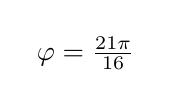
\begin{tikzpicture}
		\node at (0,0) {$\varphi=\frac{21\pi}{16}$};
		\end{tikzpicture}\\
		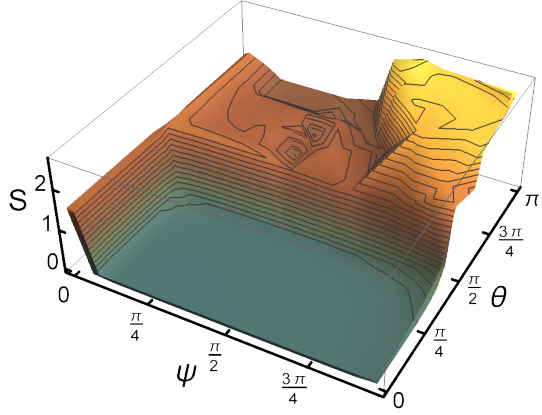
\includegraphics[width=1\textwidth]{data/Plots/Plot21.pdf}
	\end{figure}
\end{minipage}
\vspace{10pt}

\noindent
\begin{minipage}{0.48\textwidth}
	\centering
	\begin{figure}[H]
		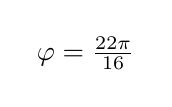
\begin{tikzpicture}
		\node at (0,0) {$\varphi=\frac{22\pi}{16}$};
		\end{tikzpicture}\\
		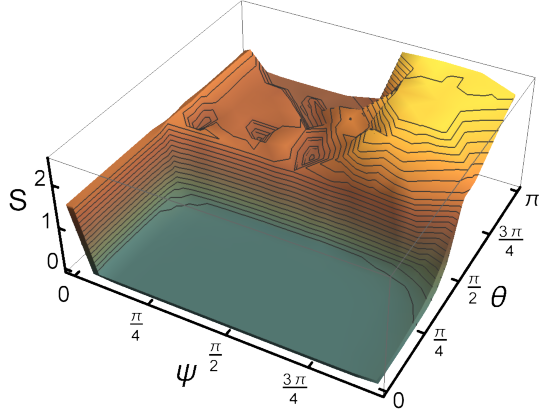
\includegraphics[width=1\textwidth]{data/Plots/Plot22.pdf}
	\end{figure}
\end{minipage}\hspace{10pt}
\begin{minipage}{0.48\textwidth}
	\centering
	\begin{figure}[H]
		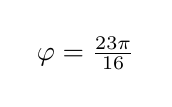
\begin{tikzpicture}
		\node at (0,0) {$\varphi=\frac{23\pi}{16}$};
		\end{tikzpicture}\\
		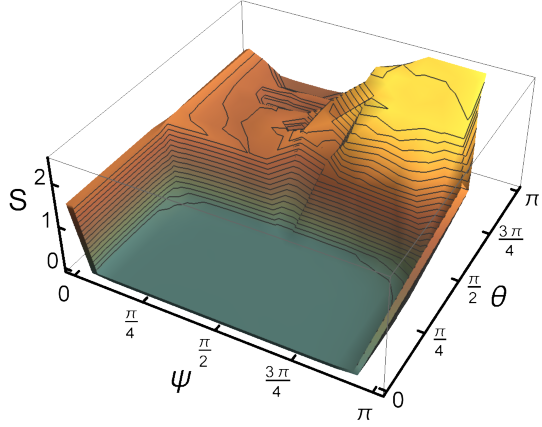
\includegraphics[width=1\textwidth]{data/Plots/Plot23.pdf}
	\end{figure}
\end{minipage}
\vspace{10pt}

\noindent
\begin{minipage}{0.48\textwidth}
	\centering
	\begin{figure}[H]
		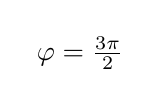
\begin{tikzpicture}
		\node at (0,0) {$\varphi=\frac{3\pi}{2}$};
		\end{tikzpicture}\\
		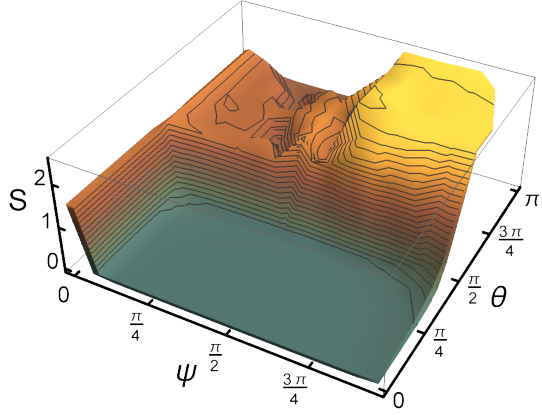
\includegraphics[width=1\textwidth]{data/Plots/Plot24.pdf}
	\end{figure}
\end{minipage}\hspace{10pt}
\begin{minipage}{0.48\textwidth}
	\centering
	\begin{figure}[H]
		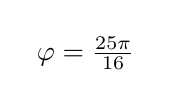
\begin{tikzpicture}
		\node at (0,0) {$\varphi=\frac{25\pi}{16}$};
		\end{tikzpicture}\\
		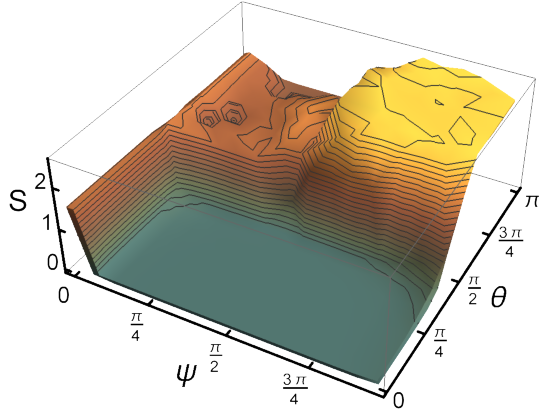
\includegraphics[width=1\textwidth]{data/Plots/Plot25.pdf}
	\end{figure}
\end{minipage}
\vspace{10pt}

\noindent
\begin{minipage}{0.48\textwidth}
	\centering
	\begin{figure}[H]
		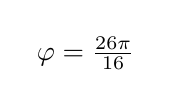
\begin{tikzpicture}
		\node at (0,0) {$\varphi=\frac{26\pi}{16}$};
		\end{tikzpicture}\\
		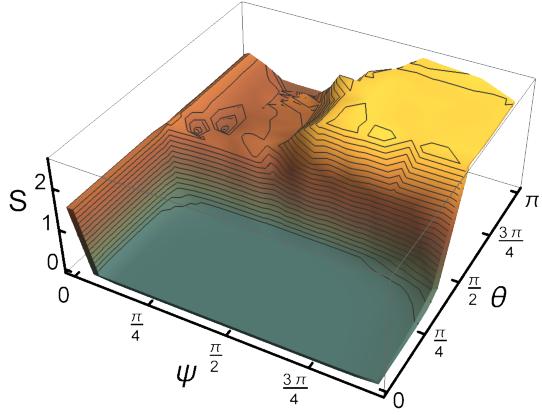
\includegraphics[width=1\textwidth]{data/Plots/Plot26.pdf}
	\end{figure}
\end{minipage}\hspace{10pt}
\begin{minipage}{0.48\textwidth}
	\centering
	\begin{figure}[H]
		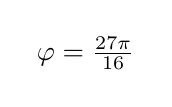
\begin{tikzpicture}
		\node at (0,0) {$\varphi=\frac{27\pi}{16}$};
		\end{tikzpicture}\\
		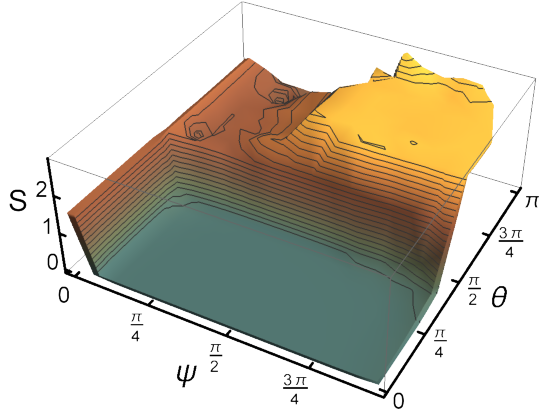
\includegraphics[width=1\textwidth]{data/Plots/Plot27.pdf}
	\end{figure}
\end{minipage}
\vspace{10pt}

\noindent
\begin{minipage}{0.48\textwidth}
	\centering
	\begin{figure}[H]
		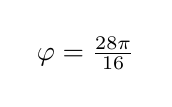
\begin{tikzpicture}
		\node at (0,0) {$\varphi=\frac{28\pi}{16}$};
		\end{tikzpicture}\\
		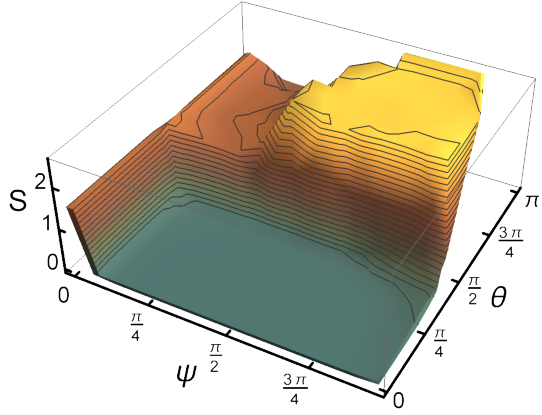
\includegraphics[width=1\textwidth]{data/Plots/Plot28.pdf}
	\end{figure}
\end{minipage}\hspace{10pt}
\begin{minipage}{0.48\textwidth}
	\centering
	\begin{figure}[H]
		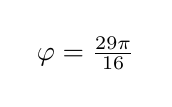
\begin{tikzpicture}
		\node at (0,0) {$\varphi=\frac{29\pi}{16}$};
		\end{tikzpicture}\\
		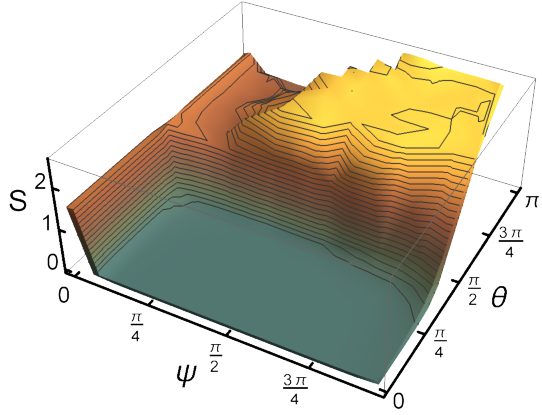
\includegraphics[width=1\textwidth]{data/Plots/Plot29.pdf}
	\end{figure}
\end{minipage}
\vspace{10pt}

\noindent
\begin{minipage}{0.48\textwidth}
	\centering
	\begin{figure}[H]
		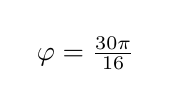
\begin{tikzpicture}
		\node at (0,0) {$\varphi=\frac{30\pi}{16}$};
		\end{tikzpicture}\\
		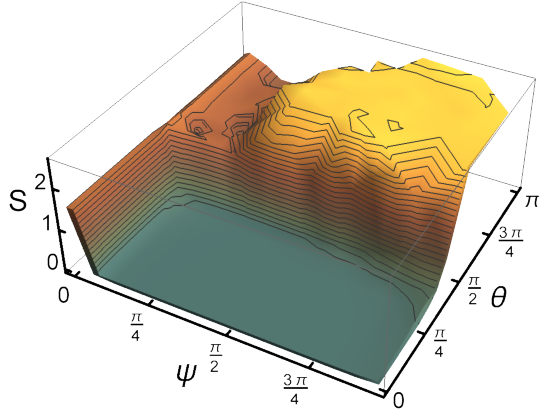
\includegraphics[width=1\textwidth]{data/Plots/Plot30.pdf}
	\end{figure}
\end{minipage}\hspace{10pt}
\begin{minipage}{0.48\textwidth}
	\centering
	\begin{figure}[H]
		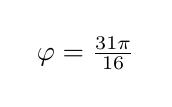
\begin{tikzpicture}
		\node at (0,0) {$\varphi=\frac{31\pi}{16}$};
		\end{tikzpicture}\\
		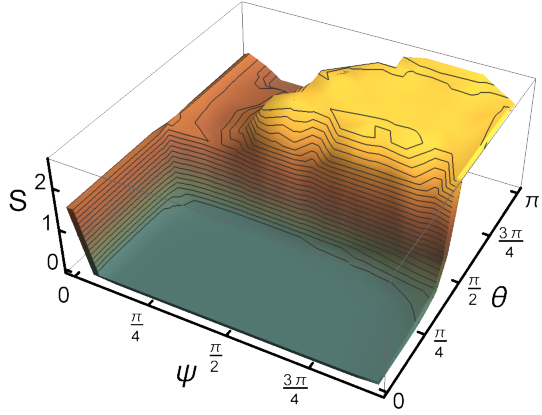
\includegraphics[width=1\textwidth]{data/Plots/Plot31.pdf}
	\end{figure}
\end{minipage}
\vspace{10pt}

\noindent
\begin{minipage}{0.48\textwidth}
	\centering
	\begin{figure}[H]
		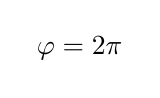
\begin{tikzpicture}
		\node at (0,0) {$\varphi=2\pi$};
		\end{tikzpicture}\\
		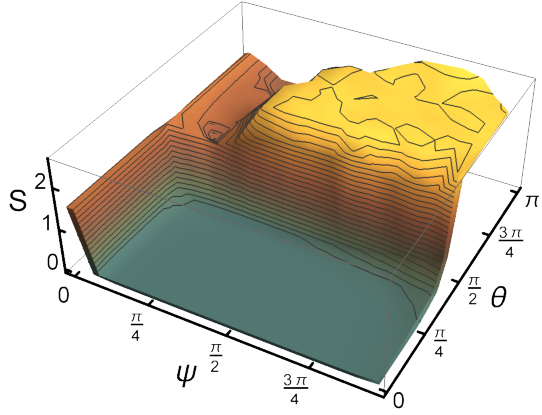
\includegraphics[width=1\textwidth]{data/Plots/Plot32.pdf}
	\end{figure}
\end{minipage}